% !TEX encoding = UTF-8 Unicode
\documentclass[11pt, a4paper, twoside, openright]{book}

% Setup of packages used
\usepackage[onehalfspacing]{setspace}		% One half spacing
\usepackage[a4paper, 					% Page Layout
                     %showframe,					% This shows the frame
                     twoside, includehead,
                     footskip=7mm, headsep=6mm,
                     top=25mm, bottom=25mm, inner=30mm, outer=25mm]{geometry}
\usepackage{sansmathfonts}				% Sans Serif equations
\renewcommand*\familydefault{\sfdefault} 		% Sans Serif as default font
\usepackage[utf8]{inputenc}				% Encoding of files: utf8
\usepackage[T1]{fontenc}					% Output font encoding for international characters

%\usepackage{fontspec}
%\setmainfont{avenirnext.ttc}[UprightFeatures={FontIndex=7},  BoldFeatures={FontIndex=5} , ItalicFeatures={FontIndex=4}, BoldItalicFeatures={FontIndex=6}]

\usepackage{titlesec}					% Redefine chapter and cahpter* titles
\titleformat{\chapter}[display]{\huge \bfseries}{\vspace{-0.5cm}\hfill \chaptertitlename\ \thechapter}{0pt}{\hfill}[{\titlerule[1.2pt]}]
\titleformat{name=\chapter,numberless}[display]{\huge \bfseries}{\vspace{-0.5cm}}{0pt}{\hfill}[{\titlerule[1.2pt]}]

% This is used to include the page number on footer within the same margins
%\titleformat{\chapter}[display]{\huge \bfseries}{\vspace{-0.5cm}\hfill \chaptertitlename\ \thechapter}{0pt}{\hfill}[{\titlerule[1.2pt] \enlargethispage{-0.75\baselineskip}}]
%\titleformat{name=\chapter,numberless}[display]{\huge \bfseries}{\vspace{-0.5cm}}{0pt}{\hfill}[{\titlerule[1.2pt] \enlargethispage{-0.75\baselineskip}}]

\usepackage{fancyhdr}					% Redefine headers
\pagestyle{fancy}
\fancyhf{}								% No header nor footer
\fancyhead[LE,RO]{\thepage}				% Left even and right odd Page Number
\fancyhead[RE]{\textit{\leftmark}}			% Right even Section
\fancyhead[LO]{\textit{\rightmark}}			% Left odd Chapter

\fancypagestyle{plain}{					% To change the footer on chapter and chapter*
	\fancyhf{}							% No header nor footer
%	\fancyfoot[C]{\vspace{-11mm}\thepage}	% Footer with number displaced
	\renewcommand{\headrulewidth}{0pt}	% No line on header
	\renewcommand{\footrulewidth}{0pt}		% No line on footer
}

\RequirePackage{caption} 				% Caption customization
\captionsetup{justification=centerlast,font=small,labelfont=sc,margin=1cm}

\usepackage{hyperref}					% Hyperlinks on pdf
\hypersetup{
    colorlinks=true,
    linkcolor=blue,
    filecolor=magenta,      
    urlcolor=blue,
    citecolor=blue,    
}

% Setup the language and its properties (choose only one)
\usepackage[spanish, es-tabla, es-nodecimaldot]{babel}
\addto\captionsspanish{\renewcommand{\contentsname}{Contenido}}
%\usepackage[english]{babel}
%\addto\captionsenglish{\renewcommand{\contentsname}{Contents}}

\usepackage{graphicx}
%\graphicspath{ {figs/} }					% Use this if custom figures folder is needed

\usepackage{amssymb,amsmath}
\usepackage[square, numbers]{natbib}		% Bibliography
\usepackage{tikz}						% Required for title page
\usetikzlibrary{babel}						% Required to make TikZ works with babel
\usepackage[section]{placeins}				% To flush floats before new section
\usepackage{longtable}				% Used by List of Symbols and friends
\usepackage{array}				% Needed by longtable package
%\nobibliography*						% To make bibliography works

% User packages, packages used in this document
\usepackage{lipsum}
\usepackage{layouts}
\printinunitsof{mm}

% Macros provided
\def\fecha{\ifcase\month\or
  Enero\or Febrero\or Marzo\or Abril\or Mayo\or Junio\or
  Julio\or Agosto\or Septiembre\or Octubre\or Noviembre\or Diciembre\fi \space\number\year
}

% User Definitions
\title{TÍTULO DEL TRABAJO}
\author{Ing. Nombre \textsc{Apellido}}
\date{\fecha}

\frontmatter
\begin{document}
\begin{titlepage}
	\onehalfspacing
	\enlargethispage{0.65\baselineskip}
	\begin{tikzpicture}[remember picture, overlay]
		\coordinate (top_right) at 
		    ([xshift=-2.5cm, yshift=-2.5cm]current page.north east);
		\coordinate (top_left) at 
		    ([xshift=2.3cm, yshift=-1.8cm]current page.north west);
		\coordinate (bottom_right) at 
		    ([xshift=-1.8cm, yshift=1.8cm]current page.south east);
		\node[inner sep=0, anchor=north east] at (top_right) {\href{http://www.itba.edu.ar}{
\includegraphics[height=19mm, trim={180 200 200 200}, clip]{figs/logo_itba.png}}};
		\draw[double, line width = 0.5pt] (top_left) rectangle (bottom_right);
	\end{tikzpicture}
	\par
%	\begin{large}
		\vspace{-0.1cm}
		\noindent \textbf{DEPARTAMENTO DE INVESTIGACIÓN Y DOCTORADO}\par
		\vspace{3cm}
		\begin{center}
			{\Huge \textbf{\@title}\par}
			{\huge \textbf{Subtítulo del trabajo (si lo hubiere)}\par}
		\end{center}
		\vfill
		\noindent \textbf{AUTOR:} \@author \par
		\vspace{1cm}
		\noindent \textbf{DIRECTOR:} Dr./Dra. Nombre \textsc{Apellido}\par
		\noindent \textbf{CO-DIRECTOR:} Dr./Dra. Nombre \textsc{Apellido}\par	
		\vspace{1cm}
		\noindent{TESIS PRESENTADA PARA LA OBTENCIÓN DEL TÍTULO DE}\par
		\noindent\textbf{DOCTOR EN INGENIERÍA / INGENIERÍA INFORMÁTICA}\par
		\vspace{1cm}
		\noindent\textbf{Comité evaluador}\par
		\begin{normalsize}		
			\noindent%
			\makebox[0.33\textwidth][l]{Dr./Dra. Nombre \textsc{Apellido}}
			\makebox[0.33\textwidth][c]{Dr./Dra. Nombre \textsc{Apellido}} 
			\makebox[0.33\textwidth][r]{Dr./Dra. Nombre \textsc{Apellido}}\par
		\end{normalsize}
		\vspace{1cm}
		\begin{center}
			\textbf{CIUDAD AUTÓNOMA DE BUENOS AIRES}\\
			\textbf{\@date}\par
		\end{center}
%	\end{large}
\end{titlepage}

% Preamble
% !TEX encoding = UTF-8 Unicode
% !TEX root = ../thesis.tex
\vspace*{0.8\textheight}
Este bla bla bla lo va a escribir Marcela \textcopyright.

% !TEX encoding = UTF-8 Unicode
% !TEX root = ../thesis.tex
\cleardoublepage
\thispagestyle{empty}
\vspace*{0.4\textheight}
\hfill A quien corresponda \par 
\vspace*{0.03\textheight}
\hfill \emph{``Cita famosa''}\par
\hfill Persona famosa ($\neq$ mí)
% !TEX encoding = UTF-8 Unicode
% !TEX root = ../thesis.tex
\chapter*{Agradecimientos}
Este espacio es opcional y puede utilizarse para agradecer a quienes han ayudado a completar este trabajo. Máximo dos hojas.
% !TEX encoding = UTF-8 Unicode
% !TEX root = ../thesis.tex
\chapter*{Resumen}
Resumen de la tesis en español. No más de 350 palabras.
% !TEX encoding = UTF-8 Unicode
% !TEX root = ../thesis.tex
\chapter*{Abstract}
Here goes the abstract of the thesis. Same restrictions as in \emph{Resumen} apply.


\tableofcontents 
\listoffigures
\listoftables
% !TEX encoding = UTF-8 Unicode
% !TEX root = ../thesis.tex
\chapter*{Símbolos y Abreviaturas}
\addcontentsline{toc}{chapter}{Abreviaturas}
\section*{Letras}
\begin{longtable}{>{\raggedright\arraybackslash}m{0.2\columnwidth}>{\raggedright\arraybackslash}m{0.8\columnwidth}}
	\textbf{Símbolo} & \textbf{Descripción} \\[0.5ex] \hline%
	\endfirsthead%
	\textbf{Símbolo} & \textbf{Descripción} \\[0.5ex] \hline%
	\endhead%
	$\mathbf{A}$ & Primer Letra del Abecedario\\
\end{longtable}

\section*{Letras Griegas}
\begin{longtable}{>{\raggedright\arraybackslash}m{0.2\columnwidth}>{\raggedright\arraybackslash}m{0.51\columnwidth}>{\centering\arraybackslash}m{0.2\columnwidth}}
	\textbf{Símbolo} & \textbf{Descripción} & \textbf{Unidades} \\[0.5ex] \hline%
	\endfirsthead%
	\textbf{Símbolo} & \textbf{Descripción} & \textbf{Unidades} \\[0.5ex] \hline%
	\endhead%
	$\pi$ & Equivalente a 3.1415... & \\
\end{longtable}

\section*{Subíndices}
\begin{longtable}{>{\raggedright\arraybackslash}m{0.2\columnwidth}>{\raggedright\arraybackslash}m{0.74\columnwidth}}
	\textbf{Subíndice} & \textbf{Descripción} \\[0.5ex] \hline%
	\endfirsthead%
	\textbf{Subíndice} & \textbf{Descripción} \\[0.5ex] \hline%
	\endhead%
	$a$ & Esto es el subíndice a\\
\end{longtable}

\section*{Superíndices}
\begin{longtable}{>{\raggedright\arraybackslash}m{0.2\columnwidth}>{\raggedright\arraybackslash}m{0.74\columnwidth}}
	\textbf{Superíndice} & \textbf{Descripción} \\[0.5ex] \hline%
	\endfirsthead%
	\textbf{Superíndice} & \textbf{Descripción} \\[0.5ex] \hline%
	\endhead%
	$\star$ & Estrellita hacia arriba\\
	$\hat{\phantom{a}}$ & Elevado a\\
	$^{o}$ & Grados Celsius\\
\end{longtable}

\section*{Abreviaturas}
\begin{longtable}{>{\raggedright\arraybackslash}m{0.2\columnwidth}>{\raggedright\arraybackslash}m{0.74\columnwidth}}
	\textbf{Abreviatura} & \textbf{Descripción} \\[0.5ex] \hline%
	\endfirsthead%
	\textbf{Abreviatura} & \textbf{Descripción} \\[0.5ex] \hline%
	\endhead%
	ITBA & \textbf{I}nstituto \textbf{T}ecnológico de \textbf{B}uenos \textbf{A}ires\\
	MIT & \textbf{M}assachusetts \textbf{I}nstitute of \textbf{T}echnology, Instituto Tecnológico de Massachusetts\\
	Cap. & \textbf{C}apítulo\\
\end{longtable}

\mainmatter
\pagenumbering{arabic}

% !TEX encoding = UTF-8 Unicode
% !TEX root = ../thesis.tex
\chapter{Introducción} \label{intro}
Este es un capítulo de ejemplo. 

Como se puede apreciar en la Fig. \ref{fig1_intro}, los lápices tienen muchos colores, los mismos se pueden generar de diversas formas \cite{ejemplo}.
\begin{figure}[htb]
	\centering
	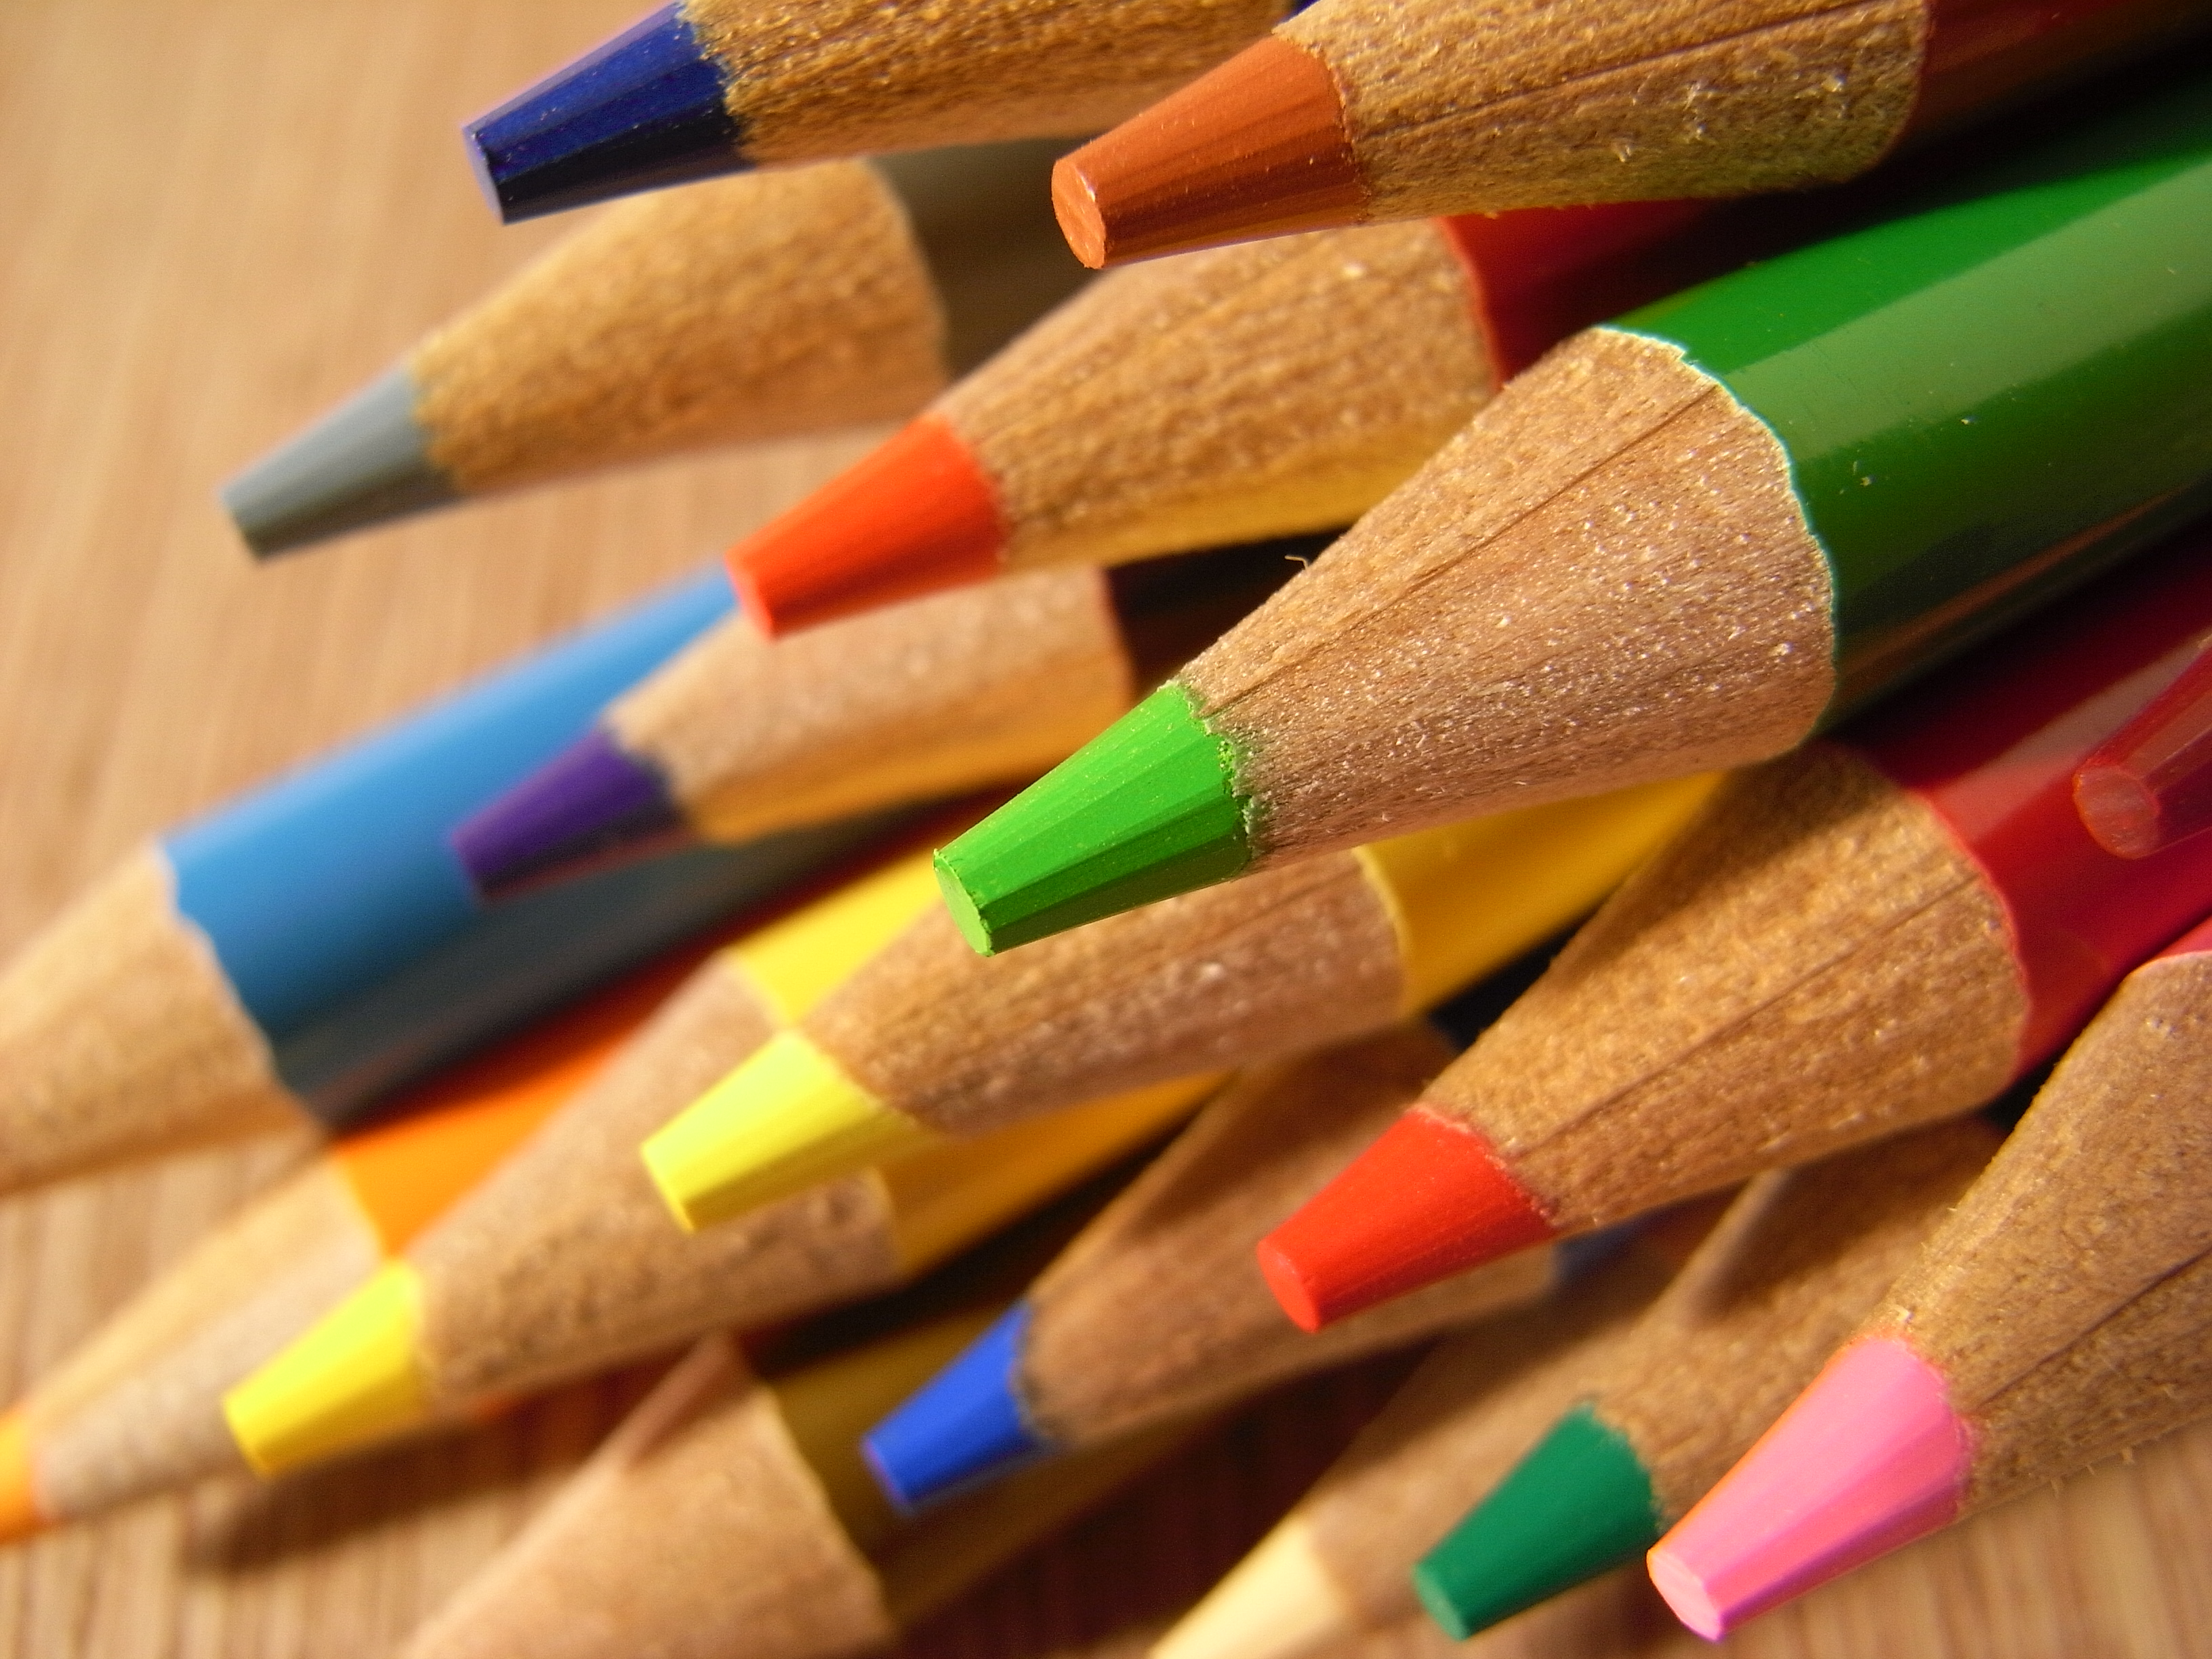
\includegraphics[width=10cm]{figs/chapter1/sample.jpg}
	\caption{Figura de ejemplo}
	\label{fig1_intro}
\end{figure}

En la Tabla \ref{table1_intro} se observan los colores disponibles.
\begin{table}[htb]
\renewcommand{\arraystretch}{1.3}
	\caption{Tabla de Colores}
	\label{table1_intro}
	\centering
	\setlength\tabcolsep{2pt}
	\begin{tabular}{c c}
		\hline
		\bfseries Código & \bfseries Color\\
		\hline
		$\mathbf{v_1}$ & Rojo\\
		$\mathbf{v_2}$ & Azul\\
		$\mathbf{v_3}$ & Verde\\
		\hline
	\end{tabular}
\end{table}

% Se agrega acá para no agregar paquetes extra al formato.
\section{Lorem Ipsum}
Lorem ipsum dolor sit amet, consectetur adipiscing elit. Pellentesque at enim at turpis vestibulum convallis. Fusce vulputate vel nunc ut ullamcorper. Nunc in dui nec lacus consectetur porttitor id feugiat ante. Interdum et malesuada fames ac ante ipsum primis in faucibus. Curabitur vulputate dui a mauris molestie, vel pulvinar urna suscipit. Sed a venenatis diam, sed faucibus felis. Vestibulum ante ipsum primis in faucibus orci luctus et ultrices posuere cubilia Curae; Proin et ullamcorper dui. Suspendisse velit nisi, malesuada et laoreet ac, consectetur sit amet justo.

Phasellus volutpat metus ut hendrerit interdum. Proin nibh purus, rutrum a ex quis, fermentum accumsan dolor. Aliquam eros tellus, blandit ac pulvinar ac, efficitur id ligula. Donec consectetur sed purus a tincidunt. Mauris consectetur enim sit amet sapien fermentum, vel ultrices lorem efficitur. Mauris ut egestas magna. Aenean non purus hendrerit, consectetur sapien a, mattis ligula. Nunc pellentesque mauris sit amet lectus accumsan, ac accumsan purus placerat. Vivamus in lacus convallis leo feugiat sodales eget vel sem. Duis finibus mi blandit felis porttitor, ac rutrum leo ultrices. Duis vel nibh ac sapien tempor laoreet. Donec a tellus et nibh ornare pulvinar sed eu justo. Morbi vulputate velit id lectus blandit mattis. Duis arcu erat, tempor a tellus sagittis, tempor dapibus tellus. Suspendisse potenti. Aliquam euismod eget arcu eu vestibulum.

Praesent libero magna, tincidunt in ante ac, mattis viverra nisl. Proin laoreet enim nisi, et scelerisque lacus aliquet non. Pellentesque habitant morbi tristique senectus et netus et malesuada fames ac turpis egestas. Cras enim massa, fringilla a pulvinar nec, sollicitudin id lorem. Etiam laoreet erat sit amet finibus tempor. Aliquam pellentesque, nisi eget luctus egestas, ligula nisi suscipit turpis, mollis cursus est ante eu nisi. Vestibulum blandit dapibus est eget mattis.

Aenean ex risus, rhoncus ut odio nec, sollicitudin imperdiet nibh. Sed efficitur congue lorem, vitae convallis mauris ornare quis. Nullam fringilla sit amet mi sed scelerisque. Quisque ac erat congue, posuere lectus ut, sollicitudin massa. Mauris quis vestibulum ante. Praesent ultrices rutrum nisi, in posuere odio fringilla ut. Nulla a mauris aliquam, dignissim mi ac, dapibus sapien. Aenean euismod at lectus quis elementum. Aenean vitae semper augue. Proin maximus odio vel mi sodales, et euismod massa lacinia. Ut venenatis nunc non urna iaculis, ac rhoncus nunc venenatis. Duis eu magna facilisis, molestie sem id, vestibulum nisl. Curabitur nec massa molestie, imperdiet turpis vitae, varius augue. Nulla scelerisque, justo sit amet eleifend mollis, urna velit venenatis sem, quis blandit arcu dolor quis est. Duis sagittis metus lacus. Praesent sed ultricies magna, in luctus massa.

Donec justo nisl, laoreet nec erat a, tempor scelerisque augue. Aliquam tempus vel enim in tempor. In nec finibus elit. Sed suscipit rhoncus nulla, id finibus est fermentum sit amet. Nunc ex lacus, laoreet placerat vulputate in, sagittis quis arcu. Vivamus sed velit ac quam blandit porttitor. Suspendisse tincidunt enim urna, eget lobortis ex posuere sed. Nam sit amet mauris ligula. Ut at vehicula sapien.

Nam suscipit finibus enim vitae elementum. Duis consequat et augue nec faucibus. Nullam imperdiet eu nunc a molestie. Proin cursus iaculis consequat. Morbi aliquet enim enim, at molestie arcu condimentum et. Sed semper erat quis iaculis eleifend. Praesent in magna et risus ultricies aliquam volutpat quis odio. In fermentum, ante a blandit iaculis, nisl velit fermentum leo, nec posuere mauris lacus id justo. Maecenas efficitur lorem sit amet leo pulvinar, a consequat eros condimentum. Suspendisse dignissim dolor sit amet magna lacinia dignissim. Vestibulum commodo velit dui, vitae hendrerit ante vehicula in. In posuere non urna a vestibulum. Donec dignissim diam eget ex porttitor pulvinar. Aenean iaculis nisl nec augue viverra, eu venenatis velit pellentesque. Nulla facilisi.

Maecenas condimentum lectus id risus sodales sodales. Curabitur fermentum ultrices posuere. Donec sed nunc eu orci molestie varius. Integer mauris ex, fringilla eu fermentum vitae, scelerisque sed est. In aliquam magna et urna elementum, a eleifend mi sollicitudin. Cras eu ipsum mauris. Orci varius natoque penatibus et magnis dis parturient montes, nascetur ridiculus mus. In tincidunt ultricies ipsum. Sed quis vestibulum neque, nec elementum lacus. Duis vitae condimentum leo, id cursus mi. Quisque bibendum libero magna, eget facilisis mi imperdiet non. Quisque viverra arcu tellus, et aliquam mauris faucibus non. Nam sagittis ut nibh a facilisis. Cras ac libero suscipit, semper leo a, blandit augue. Morbi elementum dapibus nisl, vel feugiat sem varius non.

Mauris convallis aliquam purus vitae maximus. Sed augue velit, blandit quis massa ac, vulputate tempor sem. Curabitur a auctor leo, commodo bibendum lacus. Lorem ipsum dolor sit amet, consectetur adipiscing elit. Vestibulum facilisis mi non leo suscipit malesuada. Vivamus dolor nibh, tempor quis ultrices eu, aliquam vel tellus. Integer a risus maximus, fermentum purus a, convallis neque. Aliquam ac risus nec libero suscipit rutrum ac nec nunc. Pellentesque quis scelerisque sem. Fusce faucibus lacus a lorem tincidunt commodo.

Suspendisse facilisis convallis pharetra. Cras posuere justo quis elit eleifend rhoncus. Nunc vitae nibh neque. Mauris augue massa, sagittis et magna non, condimentum tincidunt nulla. Curabitur at fringilla velit, a rutrum urna. In lacus leo, ullamcorper a auctor quis, dapibus vitae augue. Sed quis pharetra sem. Phasellus sed finibus risus. Suspendisse potenti.

Phasellus suscipit lacus sit amet elit ultrices dictum eu sed arcu. Praesent iaculis sem ut laoreet posuere. Nam vehicula pharetra hendrerit. Donec et libero ac ex posuere facilisis vel vitae ex. Aenean turpis leo, lacinia et nunc sit amet, feugiat sodales neque. Cras ultrices diam quis libero sodales gravida. Aliquam erat volutpat. Aliquam erat volutpat. Pellentesque sagittis, diam non pellentesque ultrices, massa nisi ullamcorper leo, eu tempor magna nibh eget erat.
%% !TEX encoding = UTF-8 Unicode
% !TEX root = ../thesis.tex
\chapter{Manejo Formato en \LaTeX } \label{LatexFiles}

En este capítulo se dan instrucciones generales para el manejo del formato en \LaTeX. El formato consta de diferentes archivos, que serán detallados a continuación. 

\section{Lista de Archivos}

Los archivos \textit{thesis.tex}, \textit{copyright.tex}, \textit{cover.tex}, \textit{copyright\_EN.tex} y \textit{cover\_EN.tex} corresponden a la configuración y estructura del formato del documento, y no deberían ser modificados por el usuario. En la Tabla~\ref{tab:UserFiles} se presentan la ubicación, nombre y contenido de cada archivo modificable por el usuario, donde será incluido el contenido de la tesis.

\begin{table}[ht]
\renewcommand{\arraystretch}{1.3}
    \centering
    \begin{tabular}{>{\centering}p{0.13\textwidth}p{0.19\textwidth}p{0.62\textwidth}} \hline  
    \textbf{Carpeta}  & \textbf{Archivo} & \textbf{Contenido} \\ \hline 
        & \textit{bibliography.bib} & Archivo de base de datos de las referencias bibliográficas.  \\ \hline
    \multirow{6}{*}{preamble} & \textit{abstract.tex} &  Resumen en inglés de la tesis \\ 
     & \textit{dedicatory.tex} & Dedicatoria \\  
     & \textit{resumen.tex} & Resumen en castellano de la tesis \\  
     & \textit{thanks.tex} & Agradecimientos \\  
     & \textit{title\_data.tex} & Información para la carátula de la tesis: título, autor(a), director(a), codirector(a) y jurado \\ 
     & \textit{user\_packages.tex} & Incluir paquetes específicos requeridos por el usuario. Los paquetes \textit{graphix, array, longtable} y \textit{amsmath} ya están incluidos en el formato. \\ \hline
     \multirow{2}{*}{chapters} & \textit{chapter1.tex} &  Contenido del capítulo \\ 
    & \textit{chapters\_list.tex} & Lista de capítulos a incluir en el documento. \\ \hline
    \multirow{2}{*}{appendices} & \textit{appendices\_list.tex} &  Lista de apéndices a incluir en el documento. \\ 
    & \textit{appendix1.tex} & Contenido del apéndice \\ \hline
     figs & \textit{chapter1} &  Carpeta para incluir las imágenes para el capítulo 1 \\ \hline
    \end{tabular}
    \caption{Archivos modificables por el autor}
    \label{tab:UserFiles}
\end{table}

Para quitar la portada en inglés en \LaTeX, desactive la línea \verb!% !TEX encoding = UTF-8 Unicode
% !TEX root = ../thesis.tex
\makeatletter
\begin{titlepage}
	\onehalfspacing
	\enlargethispage{0.65\baselineskip}
	\begin{tikzpicture}[remember picture, overlay]
		\coordinate (top_right) at 
		    ([xshift=-2.5cm, yshift=-2.5cm]current page.north east);
		\coordinate (top_left) at 
		    ([xshift=2.3cm, yshift=-1.8cm]current page.north west);
		\coordinate (bottom_right) at 
		    ([xshift=-1.8cm, yshift=1.8cm]current page.south east);
		\node[inner sep=0, anchor=north east] at (top_right) {\href{http://www.itba.edu.ar}{
\includegraphics[height=19mm, trim={180 200 200 200}, clip]{figs/logo_itba.png}}};
		\draw[double, line width = 0.5pt] (top_left) rectangle (bottom_right);
	\end{tikzpicture}
	\par
%	\begin{large}
		\vspace{-0.1cm}
		\noindent \textbf{DEPARTAMENTO DE INVESTIGACIÓN Y DOCTORADO}\par
		\vspace{3cm}
		\begin{center}
			{\Huge \textbf{\@titleEN}\par}
			{\huge \textbf{\@subtitleEN}\par}
		\end{center}
		\vfill
		\noindent \textbf{AUTHOR:} \@author \par
		\vspace{1cm}
		\noindent \textbf{ADVISOR:} \@director \par
		\noindent \textbf{CO-ADVISOR:} \@codirector \par	
		\vspace{1cm}
		\noindent{A THESIS SUBMITTED AS A REQUIREMENT FOR THE DEGREE OF}\par
		\noindent\textbf{\@degree}\par
		\vspace{1cm}
		\noindent\textbf{Jurado}\par
		\begin{normalsize}		
			\noindent%
			\makebox[0.33\textwidth][l]{\@firstEvaluator}
			\makebox[0.33\textwidth][c]{\@secondEvaluator} 
			\makebox[0.33\textwidth][r]{\@thirdEvaluator}\par
		\end{normalsize}
		\vspace{1cm}
		\begin{center}
			\textbf{CIUDAD AUTÓNOMA DE BUENOS AIRES}\\
			\textbf{\@dateEN}\par
		\end{center}
%	\end{large}
\end{titlepage}
% !TEX encoding = UTF-8 Unicode
% !TEX root = ../thesis.tex
\vspace*{0.8\textheight}
\noindent \@author: \@titleEN. \textit{A thesis submitted in partial fulfillment of the requirements for the degree of \textbf{\@degree} of  Instituto Tecnológico de Buenos Aires}.
\par
\vspace{1\baselineskip}
\noindent Copyright \textcopyright\space\@copyrightYear\space by Instituto Tecnológico de Buenos Aires
\makeatother! en el archivo \textit{thesis.tex} anteponiendo el símbolo de comentario (\%).

Dentro del documento, las referencias se utilizarán con estilo APA o IEEE. Para elegir el estilo, al final del archivo \textit{thesis.tex}, modifique la línea \verb!\bibliographystyle{ }! con \verb!ieeetr! para el estilo IEEE, o \verb!apalike! para APA.
%\include{chapters/chapter3}

\appendix % Next chapters are appendices
% !TEX encoding = UTF-8 Unicode
% !TEX root = ../thesis.tex
\chapter{Apéndice 1} \label{app1}
Este es un apéndice.

\textit{Esto es texto en itálica}.

\textbf{Esto es texto en negrita}.

\textsc{Esto es texto en Small Caps}

\textit{\textbf{Esto es texto en negrita itálica}}.

%\include{appendices/appendix2}

\bibliographystyle{ieeetr}
\bibliography{bibliography}
\addcontentsline{toc}{chapter}{\bibname}    %To include the bibliography in the toc

\end{document}  
